% COMPOSITE

\newpage

\subsection{Problem 4}

For the three vectors shown in the figure below,
\[
	\vec{A} + \vec{B} + \vec{C} = 1\hat{j}
	.\]
What is vector $\vec{B}$?

\begin{center}
	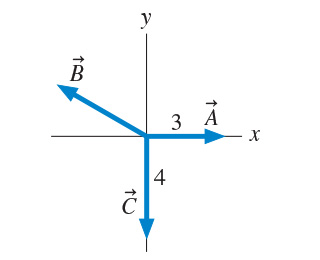
\includegraphics[width=0.5\textwidth]{/Users/max/course-manager/data/semester/Spring 2025/course/PHY2111/chapter/Vectors and Coordinate Systems/section/Quiz/figures/figure_1.jpg}
\end{center}

\setcounter{partcounter}{1}
\paragraph{Part A}

Write $\vec{B}$ in component form. Express your answer in terms of the unit vectors $\hat{i}$ and $\hat{j}$.

\begin{solution}
	We know that
	\begin{align*}
		\vec{A} &= 3\hat{i} = \left( 3, 0 \right) \\
		\vec{C} &= -4\hat{j} = \left( 0, -4 \right) \\
		\vec{V}_{\mathrm{sum}} &= \hat{j} = \left( 0, 1 \right)
		.\end{align*}
	Therefore,
	\begin{align*}
		\vec{B} &= \vec{V}_{\mathrm{sum}} - \vec{A} - \vec{C} \\
		&= \left( -3, 5 \right) = -3\hat{i} + 5\hat{j}
		.\end{align*}
\end{solution}

\setcounter{partcounter}{2}
\paragraph{Part B}

What is the magnitude of $\vec{B}$?

\begin{solution}
	\begin{align*}
		\lVert \vec{B} \rVert &= \sqrt{\left( -3 \right)^2 + 5^2} \\
		&= \sqrt{34} \\
		&\approx 5.83
		.\end{align*}
\end{solution}

\setcounter{partcounter}{3}
\paragraph{Part C}

What is the direction angle of $\vec{B}$? Express your answer in degrees.

\begin{solution}
	\begin{align*}
		\theta &= \arctan \left( \frac{5}{-3} \right) \\
		&\approx \SI{59}{\degree} ~ \text{above the negative $x$ axis}
		.\end{align*}
\end{solution}
